\chapter{Specyfikacja komponentów interfejsu do rozpoznawania emocji}
\label{cha:specyfikacja}
Celem pracy jest opracowanie prototypu interfejsu umożliwiającego pomiar sygnałów pozwalających na określenie zmian stanów emocjonalnych gracza. W związku z~tym na jeden z~elementów niniejszej pracy składa się przegląd możliwych rozwiązań użytych w~poszczególnych komponentach interfejsu. W tym rozdziale skupiono się głównie na przedstawieniu urządzeń do pomiaru sygnałów umożliwiających określenie stanu emocjonalnego użytkownika, mechanizmach wnioskowania, które mogą zostać użyte podczas budowania modelu do rozpoznawania emocji, oraz silnikach do budowy gier, przy pomocy których zostanie wykonany końcowy interfejs wraz z~grą.

\section{Platformy pomiarowe}
Pomiar sygnałów umożliwiających rozpoznawanie emocji jest jednym z~najważniejszych elementów w~pętli afektywnej. Obecnie dostępnych jest wiele platform umożliwiających wykonanie takich pomiarów i~można je podzielić na dwie główne kategorie: urządzenia służące do odczytu sygnałów fizjologicznych użytkownika oraz sprzęt, z~którego można odczytać sygnały pośrednie, na podstawie których można określić stan użytkownika.

Na pierwszą kategorię składają się między innymi platformy klasy medycznej umożliwiające dokładne pomiary odczytów z~ludzkiego ciała. Jednym z~takich urządzeń jest Neurobit Optima. Jest to przenośny sprzęt umożliwiający pomiar sygnałów takich jak praca serca, mózgu, ruchów mięśni, reakcji elektrodermalnej czy nawet temperatury skóry~\cite{neurobit_manual}. Ogromną zaletą urządzenia są wielofunkcyjne kanały pomiarowe, które użytkownik może dostosować do swoich potrzeb \cite{neurobit_manual}. Atutem, na który warto zwrócić uwagę z~perspektywy wykorzystania w~informatyce afektywnej, jest gotowe oprogramowanie dostępne od producenta oraz wbudowany interfejs Bluetooth, dzięki któremu urządzenie może być przenośne. Pomiary z~Neurobit Optima charakteryzuje wysoka dokładność i~stabilność pomiarów. Podobnym do niego urządzeniem jest NeXus-10, który podobnie jak Neurobbit Optima pozwala na pomiar pracy serca i~reakcji elektrodermalnej, posiada wbudowany interfejs Bluetooth oraz jest do niego dołączane gotowe oprogramowanie. Niestety ogromną wadą jest waga i~rozmiar urządzenia, które wpływają na wygodę podczas użytkowania. W kontekście gier afektywnych potencjalnym słabym punktem urządzeń klasy medycznej może być także ich inwazyjność. Choć w~ciągu ostatnich lat środowisko sprzętowe wyszło daleko poza standardowy komputer czy konsole, to część z~graczy może nie zaakceptować urządzeń kojarzonych z~medycyną jako części stanowiska do gier. Jednym z~problemów są tutaj szeroko wykorzystywane elektrody, które, choć umożliwiają dokładne pomiary sygnałów fizjologicznych, są kojarzone jednak głównie ze środowiskiem medycznym.

\begin{figure}
	\centering
	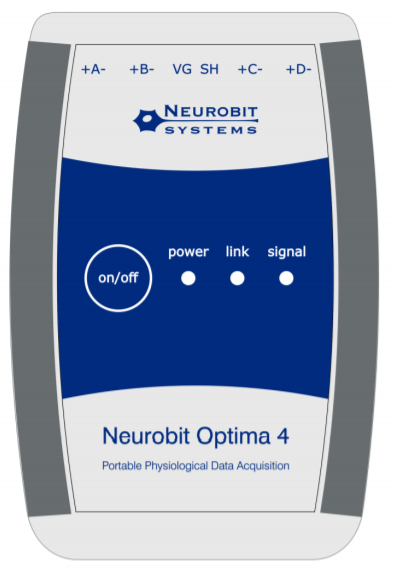
\includegraphics[width=0.3\linewidth]{images/neurobit_optima.png}
	\caption{Urządzenie Neurobit Optima, źródło: \cite{neurobit_manual}}
	\label{fig:neurobit}
\end{figure}

W kontekście platform do pomiarów sygnałów fizjologicznych w~informatyce afektywnej można zauważyć wzrost zainteresowania urządzeniami nasobnymi~\cite{wearable_sensors_2018}. Ich wyraźną zaletą jest rozmiar i~przenośność, dzięki czemu ruchy użytkownika nie są w~żadnym stopniu ograniczone. Najbardziej rozpowszechnionym, a jednocześnie jednym z~tańszych rozwiązań, są inteligentne opaski, takie jak Xiaomi Mi Band czy Microsoft Band~\cite{wearable_sensors_2018}. Oba z~wymienionych urządzeń posiadają wbudowany optyczny sensor pulsu~\cite{miband_manual,microsoft_band_factsheet}, drugie natomiast posiada także sensor do pomiaru reakcji elektrodermalnej~\cite{microsoft_band_factsheet}. Inną, mniej popularną opaską, jest Empatica E4, która poza sensorami dostępnymi w~Xiaomi Mi Band i~Microsoft Band posiada sensor do pomiaru temperatury skóry~\cite{empatica_manual}. Warto wspomnieć też o~wbudowanych w~urządzenia sensorach ruchu używanych między innymi do zliczania kroków mogących posłużyć jako sygnał pośredni, na podstawie którego można wykryć poziom aktywności użytkownika. Niestety ogromną wadą inteligentnych opasek jest ogromna niedokładność pomiarów w~porównaniu do odczytów ze sprzętów klasy medycznej. Odczyty z~opasek charakteryzują się odczytami mocno odbiegającymi od pomiarów wykonanych przy pomocy sprzętu medycznego~\cite{wearable_sensors_2018,accuracy_of_wearables_hr}.

Innymi urządzeniami nasobnymi charakteryzującymi się większą dokładnością, do których często porównuje się odczyty z~innych urządzeń do pomiaru pracy serca~\cite{wearable_sensors_2018,accuracy_of_wearables_hr}, są monitory tętna Garmin HRM-Run oraz Polar H10. W przeciwieństwie do optycznego sensora wbudowanego w~inteligentne opaski są one wyposażone w~suche elektrody wbudowane w~pasek zakładany na klatkę piersiową\cite{polar_manual,garmin_manual}. Jest to rozwiązanie, które nie jest inwazyjne dla użytkownika, a jednocześnie pozwala na dokładny pomiar pracy serca. Ważną zaletą obu urządzeń jest nie tylko wsparcie dla standardu Bluetooth, ale także dla protokołu ANT+ wykorzystywanego w~coraz większej liczbie urządzeń do pomiarów aktywności użytkownika\footnote{\textit{https://www.thisisant.com/directory}}, do którego twórcy udostępniają również gotowe implementacje interfejsów do odczytywania pomiarów, dzięki którym w~prosty sposób możliwe jest zbudowanie aplikacji interpretujących wysyłane dane.

Rozwiązaniem będącym pomostem między kosztownymi platformami medycznymi a często niedokładnymi urządzeniami nasobnymi jest platforma BITalino (r)evolution kit~\cite{bitalino_documentation}. Jest to urządzenie modułowe, składające się z~płytki stanowiącej rdzeń urządzenia, do której mogą zostać podpięte oddzielne moduły do pomiarów sygnałów fizjologicznych (rys. \ref{fig:bitalino}). Na liście dostępnych sensorów znajdują się te odpowiadające za pomiar akcji serca, reakcji elektrodermalnej skóry, czynności ruchowej mięśni oraz aktywności mózgu. Każdy z~modułów może zostać podłączony do dowolnego kanału urządzenia, natomiast pomiary odbywają się poprzez podłączenie do drugiej strony modułów kabli, na których końcu znajdują się elektrody. Co więcej, poza modułami służącymi do pomiaru reakcji fizjologicznych użytkownika, na liście dostępnych segmentów znajdują się także akcelerometr, sensor światła, dioda LED, brzęczyk, oraz przycisk, które mogą posłużyć do odczytu pomiarów pośrednich czy informowania użytkownika o~zdarzeniach. Dzięki temu platforma BITalino może służyć nie tylko jako urządzenie wykorzystywane do pomiarów, ale również do interakcji z~grą. Bardzo dużą zaletą BITalino z~perspektywy informatyki afektywnej jest dostępność narzędzi przygotowanych przez twórców, a także ogromna ilość implementacji interfejsów do komunikacji z~urządzeniem. Twórcy na swojej stronie udostępniają biblioteki dla wielu popularnych języków programowania takich jak Python, C\# czy Java, oraz konkretne implementacje z~przykładami dla środowisk takich jak silnik do gier Unity. Dodatkowym plusem jest fakt, że większość tych implementacji jest oprogramowaniem otwartym, w~związku z~czym mogą być one rozszerzane i~naprawiane przez społeczność korzystającą z~platformy.

\begin{figure}
	\centering
	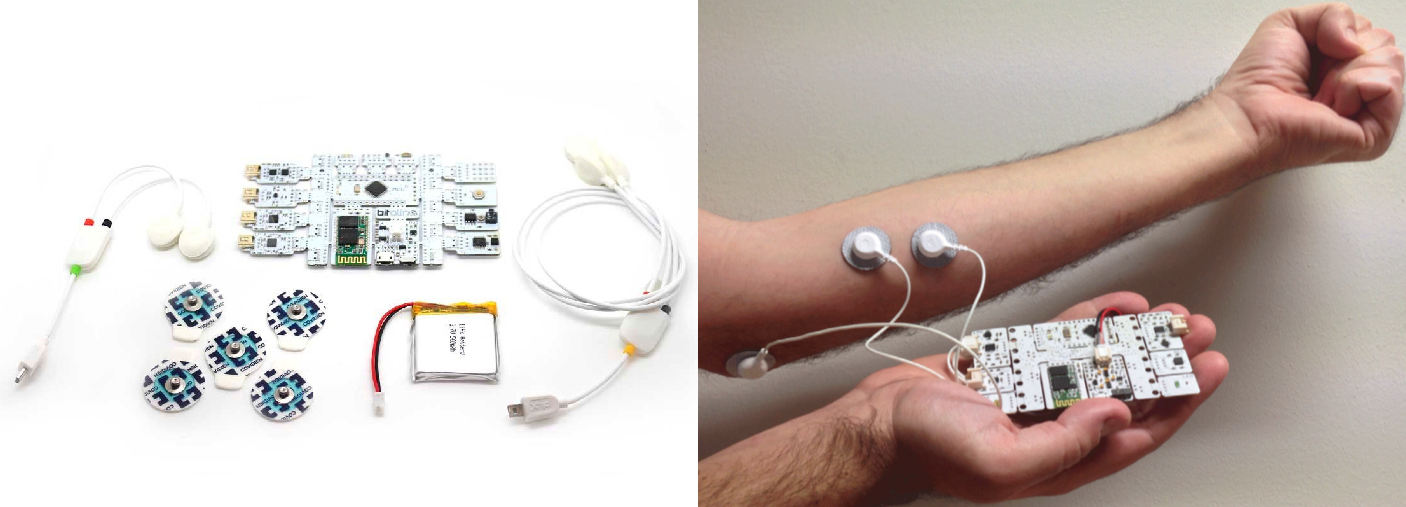
\includegraphics[width=0.9\linewidth]{images/bitalino_emg.png}
	\caption{BITalino (r)evolution kit oraz przykład podłączenia sensora do pomiaru ruchu mięśni, źródło: \cite{neurobit_manual}}
	\label{fig:bitalino}
\end{figure}

Do wspomnianej na początku drugiej kategorii urządzeń, z~których możliwe jest odczytanie sygnałów pośrednich wykorzystanych do określenia stanu użytkownika, można przede wszystkim zaliczyć sprzęty wykorzystywane przez graczy. Mowa tutaj między innymi o~myszkach, klawiaturach czy padach, z~których możliwe jest odczytanie intensywności kliknięć lub odczyt szybkości poruszania myszką na podstawie jej pozycji na ekranie~\cite{measuring_emotion_from_gamepad}. Szczególną uwagę należy poświęcić padowi Dualshock 4 od firmy Sony, który w~przeciwieństwie do większości spopularyzowanych kontrolerów do gier posiada wbudowany akcelerometr oraz żyroskop, które mogą posłużyć jako dodatkowe źródło informacji do określenia stanu emocjonalnego użytkownika~\cite{dualshock_specification}. Niestety ze względu na umowy licencyjne oprogramowanie umożliwiające odczyt tych parametrów z~pada, jest płatne, co można zaliczyć jako wadę tego rozwiązania z~perspektywy twórcy aplikacji wykorzystującej funkcjonalności Dualshocka.

\section{Możliwe mechanizmy do rozpoznawania emocji}
Opis modeli predykcji (random forest, extra trees, SVM, sieci neuronowe), krótko
\section{Narzędzia do budowy gier}
\subsection{Godot}
\subsection{Unity}
\subsection{Unreal Engine}